\section{Исследование динамики пневмопривода с использованием фазовых портретов}

Функционирование пневмопривода с дискретными распределителями характеризуется конечным
множеством возможных состояний системы, определяемых комбинациями состояний распределителей.
Математически пространство состояний распределителей может быть представлено как:

\begin{equation}\label{eq:state_space}
	\mathbf{U} = \eval{[u_1, u_2, u_3, u_4]}_{u_i} \in {0,1}, i = 1,\dots,4,
\end{equation}
где $u_i$ -- состояние i-го распределителя (0 - закрыт, 1 - открыт).
\nomenclature{$\mathbf{U}$}{Множество состояний распределителей\nomrefeqpage}
\nomenclature{$u_i$}{Состояние i-го распределителя\nomrefeqpage}

Теоретически система, как описано ранее, допускает $2^4 = 16$ различных комбинаций состояний распределителей.
Однако с учетом физических ограничений и требований безопасности целесообразно использование только определенного
подмножества состояний, формирующих основные режимы работы привода.

Классификация этих режимов представлена в таблице \ref{tab:operation_modes}.

\begin{table}[htbp]
	\centering
	\caption{Режимы работы пневматического привода с дискретными распределителями}
	\label{tab:operation_modes}
	\small
	\begin{tabular}{lcll}
		\midrule
		\textbf{Режим}           & $[u_1,u_2,u_3,u_4]$ & \textbf{Движение} & \textbf{Динамика} \\
		\midrule
		СиП\textsuperscript{1}   & $[1,0,0,1]$         &
		Максимальное положительное ускорение &
		$M\ddot{x} = p_\text{п}F_1 - p_\text{атм}F_2 - R_\text{тр}$                            \\

		СрП\textsuperscript{2}   & $[1,0,0,0]$         &
		Умеренное положительное ускорение &
		$M\ddot{x} = p_\text{п}F_1 - p_2F_2 - R_\text{тр}$                                     \\

		СлП\textsuperscript{3}   & $[0,0,0,1]$         &
		Минимальное положительное ускорение  &
		$M\ddot{x} = p_1F_1 - p_\text{атм}F_2 - R_\text{тр}$                                   \\

		СиО.\textsuperscript{4}  & $[0,1,1,0]$         &
		Максимальное отрицательное ускорение   &
		$M\ddot{x} = p_\text{атм}F_1 - p_\text{п}F_2 - R_\text{тр}$                            \\

		СрО\textsuperscript{5}   & $[0,0,1,0]$         &
		Умеренное отрицательное ускорение   &
		$M\ddot{x} = p_1F_1 - p_\text{п}F_2 - R_\text{тр}$                                     \\

		СлО\textsuperscript{6}   & $[0,1,0,0]$         &
		Минимальное отрицательное ускорение    &
		$M\ddot{x} = p_\text{атм}F_1 - p_2F_2 - R_\text{тр}$                                   \\

		\hline
		Н                        & $[0,0,0,0]$         &
		Фиксация положения       &
		$M\ddot{x} = p_1F_1 - p_2F_2 - R_\text{тр}$                                            \\
		\midrule
	\end{tabular}
	\begin{tablenotes}
		\scriptsize
		\item[1] СиП -- сильное положительное ускорение
		\item[2] СрП -- среднее положительное ускорение
		\item[3] СлП -- слабое положительное ускорение
		\item[4] СлО -- сильное отрицательное ускорение
		\item[5] СрО -- среднее отрицательное ускорение
		\item[6] СлО -- слабое отрицательное ускорение
		\item[7] Н -- удержание
	\end{tablenotes}
\end{table}

Динамическое поведение пневматического привода для каждого режима может быть
проанализировано как в пространстве давлений, так и в фазовом пространстве
скорость-положение. Векторное поле в фазовом пространстве описывается системой дифференциальных уравнений:

\begin{equation}
	\begin{cases}
		\dot{x} = v \\
		\dot{v} = \frac{1}{M}(p_1F_1 - p_2F_2 - R_\text{тр}(v))
	\end{cases}
\end{equation}
где $(x,v)$ -- координаты точки в фазовом пространстве.

В режиме сильного положительного ускорения [1,0,0,1] наблюдается максимальный
перепад давлений между полостями цилиндра, что подтверждается системой уравнений:

\begin{equation*}
	\begin{cases}
		\dot{p}_1 = \frac{\gamma RT_1}{V_1(x)}\left(G_{1,max} - \frac{p_1}{RT_1}F_1\dot{x}\right) \\
		\dot{p}_2 = \frac{\gamma RT_2}{V_2(x)}\left(-G_{4,max} + \frac{p_2}{RT_2}F_2\dot{x}\right)
	\end{cases}
\end{equation*}
где $G_{1,max}$ и $G_{4,max}$ -- максимальные массовые расходы через соответствующие распределители.

Характерной особенностью данного режима является быстрый рост давления $p_1$ до величины, близкой к давлению питания
$p_\text{п}$, с одновременным падением давления $p_2$ до атмосферного давления $p_\text{атм}$. Это обеспечивает интенсивный
разгон штока с последующим выходом на установившуюся скорость, что наглядно демонстрируется на
фазовом портрете (рис. \ref{fig:pp_strong_accelration}). Анализ фазового портрета показывает,
что процесс выхода на установившуюся скорость характеризуется движением изображающей
точки по траектории, асимптотически стремящейся к прямой $v = v_\text{уст}$.

\begin{figure}[htbp]
	\centerfloat{
		\hfill
		\subcaptionbox[List-of-Figures entry]{\label{fig:pp_strong_acceleration_positive}}{
			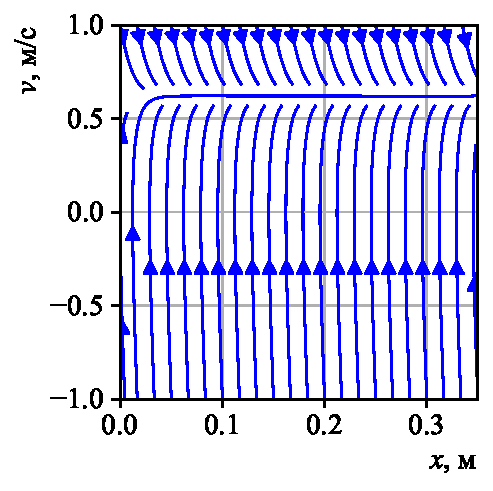
\includegraphics{part3/pp_strong_acceleration_positive.pdf} }
		\hfill
		\subcaptionbox{\label{fig:pp_strong_acceleration_negative}}{
			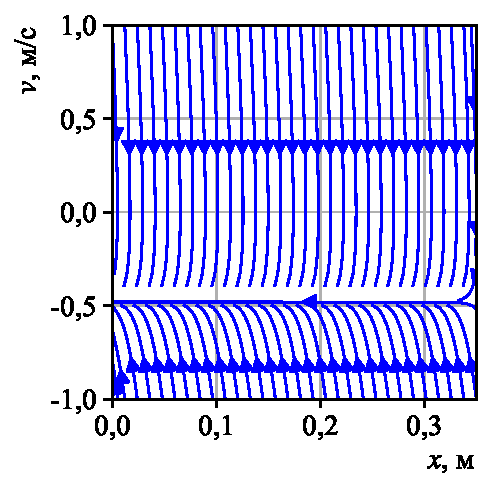
\includegraphics{part3/pp_strong_acceleration_negative.pdf} }
	}
	\caption{Фазовые портреты для режима сильного ускорения:\\
		а) положительное ускорение; б) отрицательное ускорение}
	\label{fig:pp_strong_accelration}
\end{figure}

В режимах умеренного ускорения [1,0,0,0]
наблюдается более сложная динамика, обусловленная асимметричным изменением давлений.
При данном режиме динамика давлений описывается системой:

\begin{equation}
	\begin{cases}
		\dot{p}_1 = \frac{\gamma RT_1}{V_1(x)}\left(G_{1,max} - \frac{p_1}{RT_1}F_1\dot{x}\right) \\
		\dot{p}_2 = -\frac{\gamma p_2}{V_2(x)}F_2\dot{x}
	\end{cases}
\end{equation}

Особенность данного режима заключается в том, что давление в штоковой полости изменяется согласно политропному процессу:

\begin{equation}
	p_2V_2(x)^n = p_{2,0}V_{2,0}^n = \text{const}
\end{equation}
где $p_{2,0}$ и $V_{2,0}$ -- начальное давление и объем штоковой полости соответственно в момент запирания полости;
$n$ - показатель политропы.

На фазовых портретах представленных на рисунке \ref{fig:pp_moderate_position_1} и рисунке \ref{fig:pp_moderate_position_2}
отчетливо видно влияние начальных условий на динамику системы. При большем начальном положении штока ($x_0$ равное 0,2~\si{\metre}) наблюдается более
интенсивное торможение вследствие меньшего начального объема запертой полости и, соответственно, более быстрого роста давления при сжатии воздуха.


\begin{figure}[htbp]
	\centerfloat{
		\hfill
		\subcaptionbox[List-of-Figures entry]{\label{fig:pp_medium_acceleration_x_01}}{
			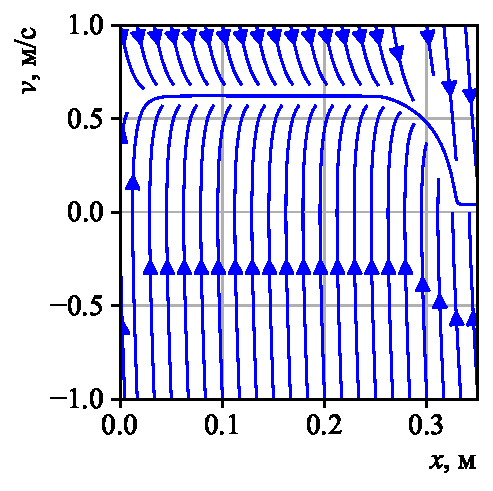
\includegraphics{part3/pp_medium_acceleration_x_01.pdf} }
		\hfill
		\subcaptionbox{\label{fig:pp_medium_acceleration_x_01_scheme}}{
			\raisebox{0.01\height}{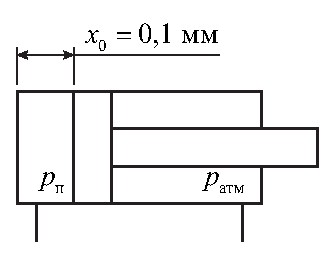
\includegraphics{part3/pp_medium_acceleration_x_01_scheme.eps}} }
	}
	\caption{Фазовый портрет и схема пневмоцилиндра при начальном положении штока $x_0 = \num{0.1}$ м ($p_{2,0} = p_\text{атм}$):\\
		а) фазовый портрет; б) схема пневмоцилиндра}
	\label{fig:pp_moderate_position_1}
\end{figure}

\begin{figure}[htbp]
	\centerfloat{
		\hfill
		\subcaptionbox[List-of-Figures entry]{\label{fig:pp_medium_acceleration_x_02}}{
			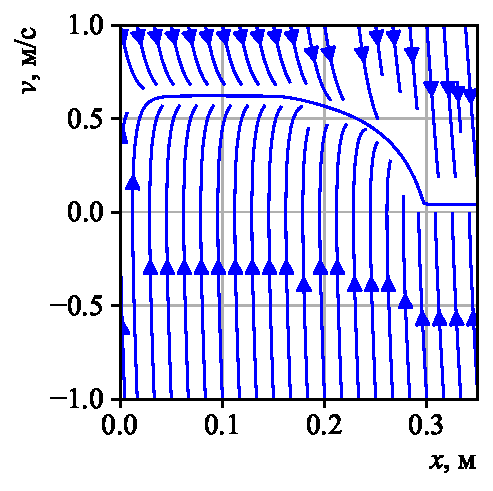
\includegraphics{part3/pp_medium_acceleration_x_02.pdf} }
		\hfill
		\subcaptionbox{\label{fig:pp_medium_acceleration_x_02_scheme}}{
			\raisebox{0.01\height}{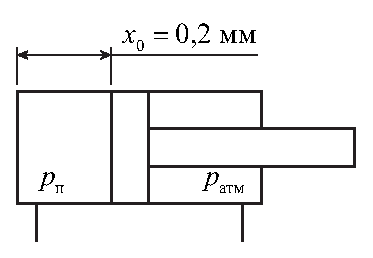
\includegraphics{part3/pp_medium_acceleration_x_02_scheme.eps}} }
	}
	\caption{Фазовый портрет и схема пневмоцилиндра при начальном положении штока $x_0 = \num{0.2}$ м ($p_{2,0} = p_\text{атм}$):\\
		а) фазовый портрет; б) схема пневмоцилиндра}
	\label{fig:pp_moderate_position_2}
\end{figure}

Для более полного понимания влияния начальных условий на динамику системы рассмотрена серия фазовых
портретов при различных комбинациях начального положения штока и давления в запираемой
полости (рис. \ref{fig:pp_moderate_matrix}). Анализ данных портретов демонстрирует, что при
фиксированном начальном положении увеличение давления $p_{2,0}$ приводит к снижению установившейся скорости
движения и увеличению интенсивности торможения. При фиксированном начальном давлении
увеличение координаты $x_0$ вызывает сокращение области достижимых состояний и смещение точки остановки к начальному положению.

\begin{figure}[htbp]
	\centerfloat{
		\hfill
		\subcaptionbox[List-of-Figures entry]{\label{fig:pp_medium_acceleration_x_01_p_2}}{
			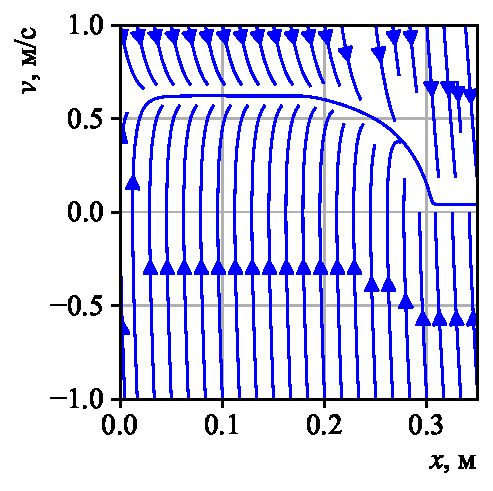
\includegraphics{part3/pp_medium_acceleration_x_01_p_2.pdf} }
		\hfill
		\subcaptionbox{\label{fig:pp_medium_acceleration_x_01_p_4}}{
			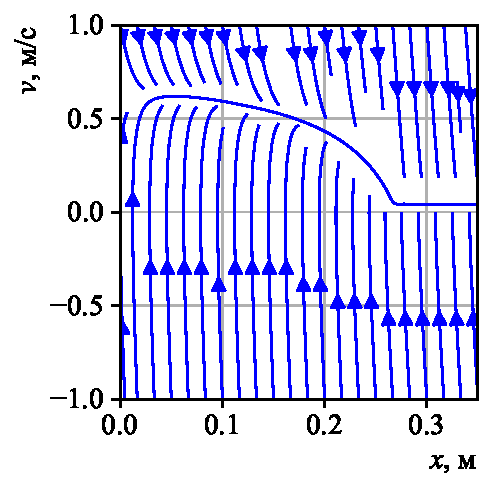
\includegraphics{part3/pp_medium_acceleration_x_01_p_4.pdf}}
		\hfill
		\subcaptionbox{\label{fig:pp_medium_acceleration_x_02_p_2}}{
			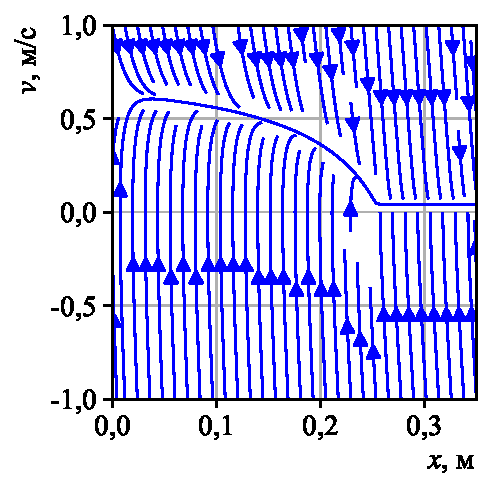
\includegraphics{part3/pp_medium_acceleration_x_02_p_2.pdf}}
		\hfill
		\subcaptionbox{\label{fig:pp_medium_acceleration_x_02_p_3}}{
			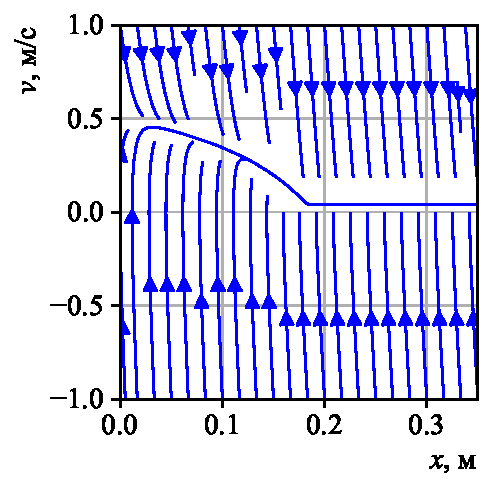
\includegraphics{part3/pp_medium_acceleration_x_02_p_4.pdf}}
	}
	\caption{Фазовые портреты при различных начальных условиях: \\
		а) $x_0 = \num{0,1}$ м, $p_{2,0} = 2$ бар; б) $x_0 = \num{0.1}$ м, $p_{2,0} = 4$ бар; \\
		в) $x_0 = \num{0.2}$ м, $p_{2,0} = 2$ бар; г) $x_0 = \num{0.2}$ м, $p_{2,0} = 4$ бар;
	}
	\label{fig:pp_moderate_matrix}
\end{figure}

Математически наблюдаемые эффекты описываются уравнением баланса сил:

\begin{equation}
	p_\text{п}F_1 - p_{2,0}\left(\frac{V_{2,0}}{V_2(x)}\right)^nF_2 = R_\text{тр}(v),
\end{equation}
где $V_2(x) = V_{2,0} + A_2(L - x)$ -- текущий объем запертой полости.

Режимы слабого ускорения [0,0,0,1] или [0,1,0,0] характеризуются минимальным перепадом давлений между
полостями пневмоцилиндра. Рассмотрим режим слабого положительного ускорения [0,0,0,1], при котором поршневая полость
изолирована, а штоковая соединена с атмосферой. Динамика давлений в данном режиме описывается системой уравнений:

$$\begin{cases}
		\dot{p}_1 = -\frac{\gamma p_1}{V_1(x)}F_1\dot{x} \\
		\dot{p}_2 = \frac{\gamma RT_2}{V_2(x)}(-G_{4,max} + \frac{p_2}{RT_2}F_2\dot{x})
	\end{cases}$$

% На графиках отображенных на рисунке \ref{fig:pressure_comparison} видно, что давление $p_2$ снижается до
% тмосферного значения существенно медленнее, чем в режиме сильного ускорения, в то время как
% давление $p_1$ изменяется только за счет изменения объема поршневой полости.
Данный процесс
характеризуется политропным изменением состояния воздуха в запертой полости:

\begin{equation}
	p_1V_1(x)^n = p_{1,0}V_{1,0}^n = \text{const}
\end{equation}
где $p_{1,0}$ и $V_{1,0}$ -- начальные значения давления и объема поршневой полости соответственно.

\begin{figure}[htbp]
	\centerfloat{
		\hfill
		\subcaptionbox[List-of-Figures entry]{\label{fig:pp_weak_acceleration_x01}}{
			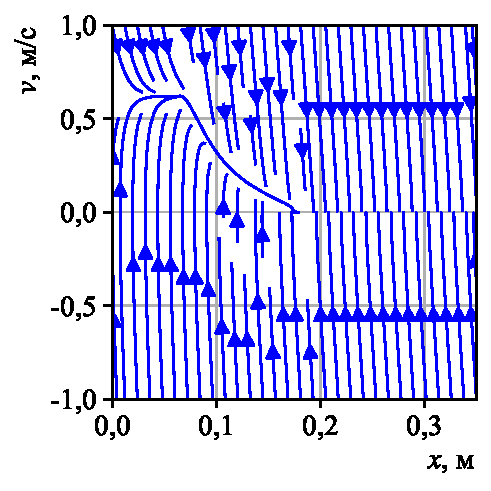
\includegraphics{part3/pp_slow_acceleration_x_01_p_3.pdf} }
		\hfill
		\subcaptionbox{\label{fig:pp_weak_acceleration_x02}}{
			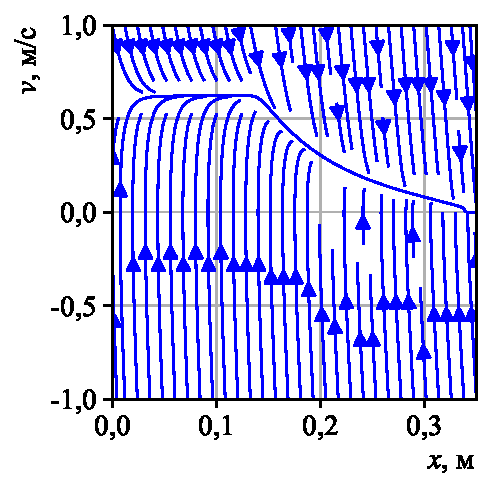
\includegraphics{part3/pp_slow_acceleration_x_02_p_3.pdf} }
	}
	\caption{Фазовые портреты для режима слабого ускорения при различных начальных условиях:\\
		а) $x_0 = \num{0.1}$ м, $p_{1,0} = 3$ бар; б) $x_0 = \num{0.2}$ м, $p_{1,0} = 3$ бар}
	\label{fig:pp_weak_acceleration}
\end{figure}

Анализ фазовых портретов представленных на рисунке \ref{fig:pp_weak_acceleration} показывает существенное влияние начального
положения штока на динамику системы. При увеличении начальной координаты $x_0$ наблюдается снижение максимально достижимой
скорости и уменьшение пути перемещения до точки остановки. Это объясняется более быстрым падением давления $p_1$ при расширении
воздуха в запертой полости большего начального объема.

Уравнение баланса сил для данного режима имеет вид:

\begin{equation}
	p_{1,0}\left(\frac{V_{1,0}}{V_1(x)}\right)^nF_1 - p_\text{атм}F_2 = R_\text{тр}(v)
\end{equation}
где $V_1(x) = V_{1,0} + A_1x$ - текущий объем поршневой полости.

Характерной особенностью режима слабого ускорения является существенная зависимость динамики
от сил трения. На фазовых портретах это проявляется в виде более крутых траекторий
торможения и меньшей области достижимых состояний по сравнению с режимами сильного и
умеренного ускорения. Данный эффект объясняется тем, что движущая сила, определяемая
разностью давлений в полостях, сопоставима по величине с силами трения.

Для оценки влияния начального давления в запертой полости на динамику системы рассмотрим
серию фазовых портретов при различных значениях $p_{1,0}$ приведенных на рисунке \ref{fig:pp_weak_pressure_matrix}.

\begin{figure}[htbp]
	\centerfloat{
		\hfill
		\subcaptionbox[List-of-Figures entry]{\label{fig:pp_weak_p2}}{
			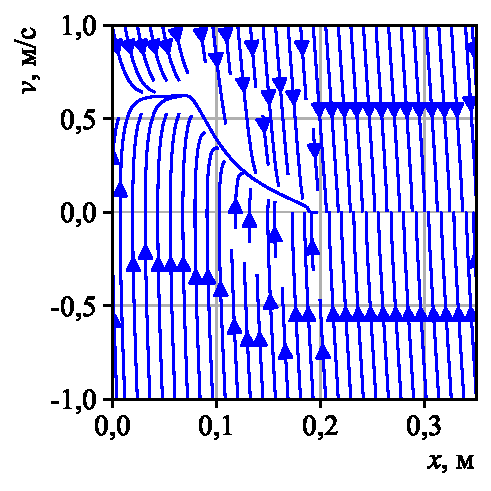
\includegraphics{part3/pp_slow_acceleration_x_015_p_2.pdf} }
		\hfill
		\subcaptionbox{\label{fig:pp_weak_p3}}{
			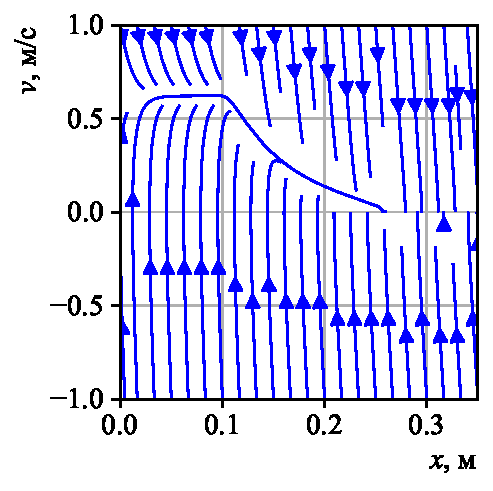
\includegraphics{part3/pp_slow_acceleration_x_015_p_3.pdf} }
		\vfill
		\subcaptionbox{\label{fig:pp_weak_p4}}{
			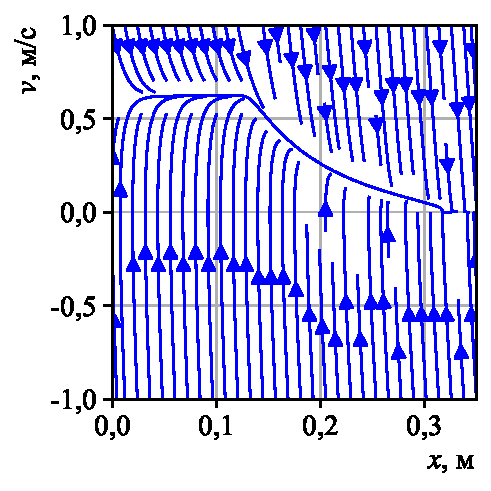
\includegraphics{part3/pp_slow_acceleration_x_015_p_4.pdf} }
	}
	\caption{Фазовые портреты при $x_0 = \num{0.15}$ м и различных начальных давлениях:\\
		а) $p_{1,0} = 2$ бар; б) $p_{1,0} = 3$ бар; в) $p_{1,0} = 4$ бар}
	\label{fig:pp_weak_pressure_matrix}
\end{figure}

Анализ представленных фазовых портретов демонстрирует, что увеличение начального давления $p_{1,0}$ приводит
к возрастанию максимальной скорости движения и увеличению дальности перемещения штока. При этом форма
фазовых траекторий становится более пологой, что свидетельствует о меньшем влиянии сил трения
на динамику системы. Данный эффект объясняется увеличением движущей силы при сохранении характера
её изменения в процессе движения.

%%%%%%%%%%%%%%%%%%%%%%%% mode 0

Режим удержания [0,0,0,0] представляет особый интерес с точки зрения
динамики электропневматического привода, поскольку в данном режиме обе полости
пневмоцилиндра оказываются изолированными.Изменение давлений при этом
происходит исключительно за счет изменения объемов полостей и описывается системой уравнений:

$$\begin{cases}
		\dot{p}_1 = -\frac{\gamma p_1}{V_1(x)}F_1\dot{x} \\
		\dot{p}_2 = -\frac{\gamma p_2}{V_2(x)}F_2\dot{x}
	\end{cases}$$

% На графиках изменения давлений, согласно рисунку \ref{fig:pressure_comparison}, 

В данном режиме наблюдается характерное
политропное изменение состояния воздуха в обеих полостях, описываемое уравнениями:

\begin{equation}
	\begin{cases}
		p_1V_1(x)^n = p_{1,0}V_{1,0}^n = \text{const} \\
		p_2V_2(x)^n = p_{2,0}V_{2,0}^n = \text{const}
	\end{cases}
\end{equation}
где $p_{1,0}$, $V_{1,0}$ и $p_{2,0}$, $V_{2,0}$ -- начальные значения давлений и объемов поршневой и штоковой полостей соответственно.

Стабилизация положения штока в режиме удержания обеспечивается преимущественно силами трения, а также дополнительно
поддерживается пневматической жёсткостью, создаваемой сжатым воздухом в изолированных полостях. Баланс сил в данном режиме описывается уравнением:

\begin{equation}
	p_1F_1 - p_2F_2 = R_\text{тр}(v)
\end{equation}

\begin{figure}[htbp]
	\centerfloat{
		\hfill
		\subcaptionbox[List-of-Figures entry]{\label{fig:pp_hold_low_pressure}}{
			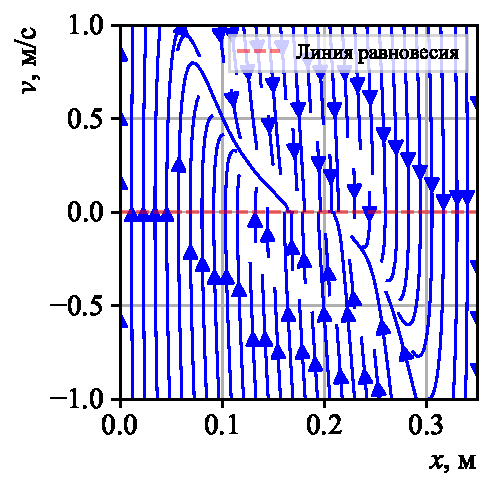
\includegraphics{part3/pp_hold_low_pressure.pdf} }
		\hfill
		\subcaptionbox{\label{fig:pp_hold_high_pressure}}{
			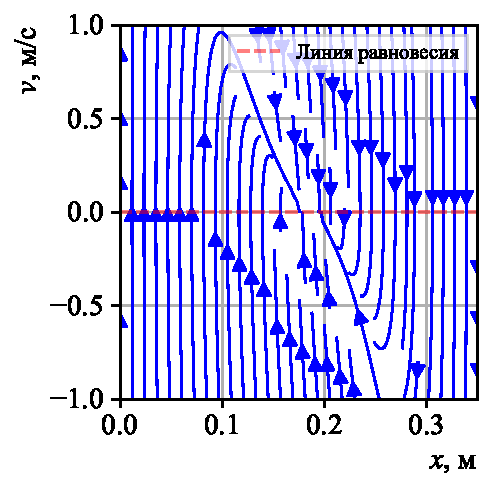
\includegraphics{part3/pp_hold_high_pressure.pdf} }
	}
	\caption{Фазовые портреты для режима удержания при различных начальных давлениях:\\
		а) низкие начальные давления ($p_{1,0} = 2$ бар, $p_{2,0} = \num{2}$ бар);\\
		б) высокие начальные давления ($p_{1,0} = 4$ бар, $p_{2,0} = \num{4}$ бар)}
	\label{fig:pp_hold_mode}
\end{figure}

Анализ фазовых портретов для режима удержания показанных на рисунке \ref{fig:pp_hold_mode} показывает высокую эффективность удержания положения штока при различных начальных давлениях.
В системе наблюдается апериодический характер движения с быстрым затуханием скорости, что обусловлено существенным влиянием сил трения.
При этом уровень начальных давлений в полостях оказывает незначительное влияние на характер переходного процесса, что подтверждается схожей формой фазовых траекторий.

\begin{figure}[htbp]
	\centerfloat{
		\hfill
		\subcaptionbox[List-of-Figures entry]{\label{fig:pp_hold_balanced}}{
			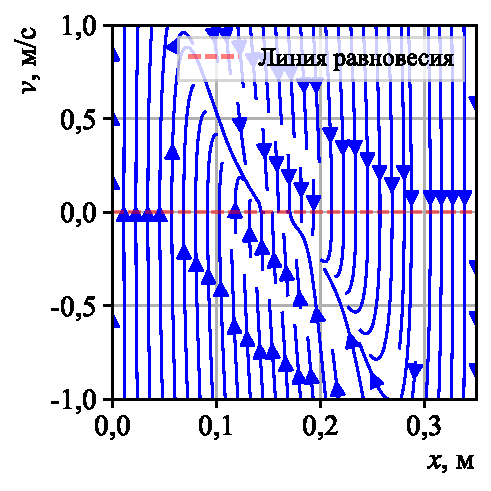
\includegraphics{part3/pp_hold_balanced.pdf} }
		\hfill
		\subcaptionbox{\label{fig:pp_hold_unbalanced}}{
			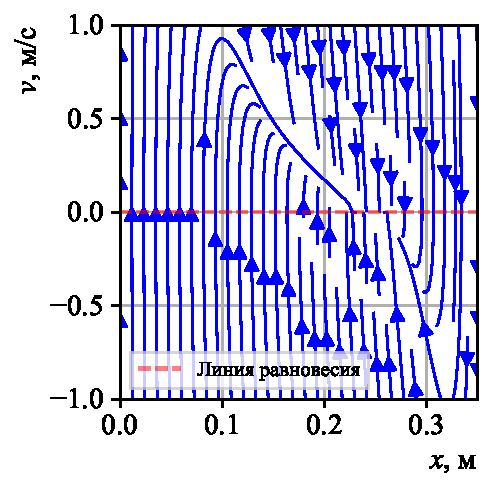
\includegraphics{part3/pp_hold_unbalanced.pdf} }
	}
	\caption{Фазовые портреты при $x_0 = \num{0.15}$ м и различных соотношениях начальных давлений:\\
		а) близкие давления ($p_{1,0} = 3$ бар, $p_{2,0} = 3$ бар);\\
		б) существенная разница ($p_{1,0} = 2$ бар, $p_{2,0} = 4$ бар)}
	\label{fig:pp_hold_matrix}
\end{figure}

Рассмотрение фазовых портретов при различных соотношениях начальных давлений отображенных на  рисунке \ref{fig:pp_hold_matrix} демонстрирует,
что даже при значительной разнице давлений в полостях система сохраняет устойчивое апериодическое движение к положению равновесия.
При близких значениях давлений $p_{1,0}$ и $p_{2,0}$ наблюдается симметричный характер фазовых траекторий. Увеличение разности давлений приводит к незначительной асимметрии траекторий при сохранении общего характера движения.

Математическое описание движения в окрестности положения равновесия может быть получено линеаризацией уравнений движения:

\begin{equation}
	M\ddot{x} + \left(\frac{\gamma p_{1,0}F_1^2}{V_{1,0}} + \frac{\gamma p_{2,0}F_2^2}{V_{2,0}}\right)x + \nu\dot{x} = 0
\end{equation}
где $\nu$ -- коэффициент вязкого трения. Существенное преобладание силы трения над пневматической жёсткостью
($\nu \gg \sqrt{M\left(\frac{\gamma p_{1,0}F_1^2}{V_{1,0}} + \frac{\gamma p_{2,0}F_2^2}{V_{2,0}}\right)}$) обуславливает апериодический характер движения системы.
\nomenclature{$\nu$}{Коэффициент вязкого трения\nomrefeqpage}

Проведенный анализ режимов работы электропневматического привода с дискретными распределителями
позволил выявить характерные особенности динамики системы для каждого режима функционирования.
В режиме сильного ускорения [1,0,0,1] наблюдается максимальный перепад давлений между полостями и,
как следствие, наибольшая интенсивность разгона штока с последующим выходом на установившуюся скорость.
Режим умеренного ускорения [1,0,0,0] характеризуется существенным влиянием начальных условий на динамику
системы вследствие политропного изменения состояния воздуха в запертой полости. Режим слабого ускорения
[0,0,0,1] демонстрирует значительную зависимость от сил трения при минимальном перепаде давлений между полостями.
Особую роль играет режим удержания [0,0,0,0], в котором стабилизация положения штока обеспечивается преимущественно
силами трения при апериодическом характере затухания скорости. Построенные фазовые портреты и анализ динамики давлений
позволяют научно обоснованно подходить к выбору режимов работы при проектировании алгоритмов управления электропневматическим
приводом с дискретными распределителями. При этом учет выявленных закономерностей и особенностей каждого режима позволяет
обеспечить требуемые показатели качества позиционирования при минимизации количества переключений распределителей.